
%% bare_conf.tex
%% V1.4b
%% 2015/08/26
%% by Michael Shell
%% See:
%% http://www.michaelshell.org/
%% for current contact information.
%%
%% This is a skeleton file demonstrating the use of IEEEtran.cls
%% (requires IEEEtran.cls version 1.8b or later) with an IEEE
%% conference paper.
%%
%% Support sites:
%% http://www.michaelshell.org/tex/ieeetran/
%% http://www.ctan.org/pkg/ieeetran
%% and
%% http://www.ieee.org/

%%*************************************************************************
%% Legal Notice:
%% This code is offered as-is without any warranty either expressed or
%% implied; without even the implied warranty of MERCHANTABILITY or
%% FITNESS FOR A PARTICULAR PURPOSE! 
%% User assumes all risk.
%% In no event shall the IEEE or any contributor to this code be liable for
%% any damages or losses, including, but not limited to, incidental,
%% consequential, or any other damages, resulting from the use or misuse
%% of any information contained here.
%%
%% All comments are the opinions of their respective authors and are not
%% necessarily endorsed by the IEEE.
%%
%% This work is distributed under the LaTeX Project Public License (LPPL)
%% ( http://www.latex-project.org/ ) version 1.3, and may be freely used,
%% distributed and modified. A copy of the LPPL, version 1.3, is included
%% in the base LaTeX documentation of all distributions of LaTeX released
%% 2003/12/01 or later.
%% Retain all contribution notices and credits.
%% ** Modified files should be clearly indicated as such, including  **
%% ** renaming them and changing author support contact information. **
%%*************************************************************************


% *** Authors should verify (and, if needed, correct) their LaTeX system  ***
% *** with the testflow diagnostic prior to trusting their LaTeX platform ***
% *** with production work. The IEEE's font choices and paper sizes can   ***
% *** trigger bugs that do not appear when using other class files.       ***                          ***
% The testflow support page is at:
% http://www.michaelshell.org/tex/testflow/



\documentclass[conference]{IEEEtran}
% Some Computer Society conferences also require the compsoc mode option,
% but others use the standard conference format.
%
% If IEEEtran.cls has not been installed into the LaTeX system files,
% manually specify the path to it like:
% \documentclass[conference]{../sty/IEEEtran}





% Some very useful LaTeX packages include:
% (uncomment the ones you want to load)


% *** MISC UTILITY PACKAGES ***
%
%\usepackage{ifpdf}
% Heiko Oberdiek's ifpdf.sty is very useful if you need conditional
% compilation based on whether the output is pdf or dvi.
% usage:
% \ifpdf
%   % pdf code
% \else
%   % dvi code
% \fi
% The latest version of ifpdf.sty can be obtained from:
% http://www.ctan.org/pkg/ifpdf
% Also, note that IEEEtran.cls V1.7 and later provides a builtin
% \ifCLASSINFOpdf conditional that works the same way.
% When switching from latex to pdflatex and vice-versa, the compiler may
% have to be run twice to clear warning/error messages.






% *** CITATION PACKAGES ***
%
%\usepackage{cite}
% cite.sty was written by Donald Arseneau
% V1.6 and later of IEEEtran pre-defines the format of the cite.sty package
% \cite{} output to follow that of the IEEE. Loading the cite package will
% result in citation numbers being automatically sorted and properly
% "compressed/ranged". e.g., [1], [9], [2], [7], [5], [6] without using
% cite.sty will become [1], [2], [5]--[7], [9] using cite.sty. cite.sty's
% \cite will automatically add leading space, if needed. Use cite.sty's
% noadjust option (cite.sty V3.8 and later) if you want to turn this off
% such as if a citation ever needs to be enclosed in parenthesis.
% cite.sty is already installed on most LaTeX systems. Be sure and use
% version 5.0 (2009-03-20) and later if using hyperref.sty.
% The latest version can be obtained at:
% http://www.ctan.org/pkg/cite
% The documentation is contained in the cite.sty file itself.






% *** GRAPHICS RELATED PACKAGES ***
%
\ifCLASSINFOpdf
   \usepackage[pdftex]{graphicx}
  % declare the path(s) where your graphic files are
  % \graphicspath{{../pdf/}{../jpeg/}}
  % and their extensions so you won't have to specify these with
  % every instance of \includegraphics
  % \DeclareGraphicsExtensions{.pdf,.jpeg,.png}
\else
  % or other class option (dvipsone, dvipdf, if not using dvips). graphicx
  % will default to the driver specified in the system graphics.cfg if no
  % driver is specified.
  % \usepackage[dvips]{graphicx}
  % declare the path(s) where your graphic files are
  % \graphicspath{{../eps/}}
  % and their extensions so you won't have to specify these with
  % every instance of \includegraphics
  % \DeclareGraphicsExtensions{.eps}
\fi
% graphicx was written by David Carlisle and Sebastian Rahtz. It is
% required if you want graphics, photos, etc. graphicx.sty is already
% installed on most LaTeX systems. The latest version and documentation
% can be obtained at: 
% http://www.ctan.org/pkg/graphicx
% Another good source of documentation is "Using Imported Graphics in
% LaTeX2e" by Keith Reckdahl which can be found at:
% http://www.ctan.org/pkg/epslatex
%
% latex, and pdflatex in dvi mode, support graphics in encapsulated
% postscript (.eps) format. pdflatex in pdf mode supports graphics
% in .pdf, .jpeg, .png and .mps (metapost) formats. Users should ensure
% that all non-photo figures use a vector format (.eps, .pdf, .mps) and
% not a bitmapped formats (.jpeg, .png). The IEEE frowns on bitmapped formats
% which can result in "jaggedy"/blurry rendering of lines and letters as
% well as large increases in file sizes.
%
% You can find documentation about the pdfTeX application at:
% http://www.tug.org/applications/pdftex





% *** MATH PACKAGES ***
%
%\usepackage{amsmath}
% A popular package from the American Mathematical Society that provides
% many useful and powerful commands for dealing with mathematics.
%
% Note that the amsmath package sets \interdisplaylinepenalty to 10000
% thus preventing page breaks from occurring within multiline equations. Use:
%\interdisplaylinepenalty=2500
% after loading amsmath to restore such page breaks as IEEEtran.cls normally
% does. amsmath.sty is already installed on most LaTeX systems. The latest
% version and documentation can be obtained at:
% http://www.ctan.org/pkg/amsmath





% *** SPECIALIZED LIST PACKAGES ***
%
%\usepackage{algorithmic}
% algorithmic.sty was written by Peter Williams and Rogerio Brito.
% This package provides an algorithmic environment fo describing algorithms.
% You can use the algorithmic environment in-text or within a figure
% environment to provide for a floating algorithm. Do NOT use the algorithm
% floating environment provided by algorithm.sty (by the same authors) or
% algorithm2e.sty (by Christophe Fiorio) as the IEEE does not use dedicated
% algorithm float types and packages that provide these will not provide
% correct IEEE style captions. The latest version and documentation of
% algorithmic.sty can be obtained at:
% http://www.ctan.org/pkg/algorithms
% Also of interest may be the (relatively newer and more customizable)
% algorithmicx.sty package by Szasz Janos:
% http://www.ctan.org/pkg/algorithmicx




% *** ALIGNMENT PACKAGES ***
%
%\usepackage{array}
% Frank Mittelbach's and David Carlisle's array.sty patches and improves
% the standard LaTeX2e array and tabular environments to provide better
% appearance and additional user controls. As the default LaTeX2e table
% generation code is lacking to the point of almost being broken with
% respect to the quality of the end results, all users are strongly
% advised to use an enhanced (at the very least that provided by array.sty)
% set of table tools. array.sty is already installed on most systems. The
% latest version and documentation can be obtained at:
% http://www.ctan.org/pkg/array


% IEEEtran contains the IEEEeqnarray family of commands that can be used to
% generate multiline equations as well as matrices, tables, etc., of high
% quality.




% *** SUBFIGURE PACKAGES ***
%\ifCLASSOPTIONcompsoc
%  \usepackage[caption=false,font=normalsize,labelfont=sf,textfont=sf]{subfig}
%\else
%  \usepackage[caption=false,font=footnotesize]{subfig}
%\fi
% subfig.sty, written by Steven Douglas Cochran, is the modern replacement
% for subfigure.sty, the latter of which is no longer maintained and is
% incompatible with some LaTeX packages including fixltx2e. However,
% subfig.sty requires and automatically loads Axel Sommerfeldt's caption.sty
% which will override IEEEtran.cls' handling of captions and this will result
% in non-IEEE style figure/table captions. To prevent this problem, be sure
% and invoke subfig.sty's "caption=false" package option (available since
% subfig.sty version 1.3, 2005/06/28) as this is will preserve IEEEtran.cls
% handling of captions.
% Note that the Computer Society format requires a larger sans serif font
% than the serif footnote size font used in traditional IEEE formatting
% and thus the need to invoke different subfig.sty package options depending
% on whether compsoc mode has been enabled.
%
% The latest version and documentation of subfig.sty can be obtained at:
% http://www.ctan.org/pkg/subfig




% *** FLOAT PACKAGES ***
%
%\usepackage{fixltx2e}
% fixltx2e, the successor to the earlier fix2col.sty, was written by
% Frank Mittelbach and David Carlisle. This package corrects a few problems
% in the LaTeX2e kernel, the most notable of which is that in current
% LaTeX2e releases, the ordering of single and double column floats is not
% guaranteed to be preserved. Thus, an unpatched LaTeX2e can allow a
% single column figure to be placed prior to an earlier double column
% figure.
% Be aware that LaTeX2e kernels dated 2015 and later have fixltx2e.sty's
% corrections already built into the system in which case a warning will
% be issued if an attempt is made to load fixltx2e.sty as it is no longer
% needed.
% The latest version and documentation can be found at:
% http://www.ctan.org/pkg/fixltx2e


%\usepackage{stfloats}
% stfloats.sty was written by Sigitas Tolusis. This package gives LaTeX2e
% the ability to do double column floats at the bottom of the page as well
% as the top. (e.g., "\begin{figure*}[!b]" is not normally possible in
% LaTeX2e). It also provides a command:
%\fnbelowfloat
% to enable the placement of footnotes below bottom floats (the standard
% LaTeX2e kernel puts them above bottom floats). This is an invasive package
% which rewrites many portions of the LaTeX2e float routines. It may not work
% with other packages that modify the LaTeX2e float routines. The latest
% version and documentation can be obtained at:
% http://www.ctan.org/pkg/stfloats
% Do not use the stfloats baselinefloat ability as the IEEE does not allow
% \baselineskip to stretch. Authors submitting work to the IEEE should note
% that the IEEE rarely uses double column equations and that authors should try
% to avoid such use. Do not be tempted to use the cuted.sty or midfloat.sty
% packages (also by Sigitas Tolusis) as the IEEE does not format its papers in
% such ways.
% Do not attempt to use stfloats with fixltx2e as they are incompatible.
% Instead, use Morten Hogholm'a dblfloatfix which combines the features
% of both fixltx2e and stfloats:
%
% \usepackage{dblfloatfix}
% The latest version can be found at:
% http://www.ctan.org/pkg/dblfloatfix




% *** PDF, URL AND HYPERLINK PACKAGES ***
%
\usepackage{url}
% url.sty was written by Donald Arseneau. It provides better support for
% handling and breaking URLs. url.sty is already installed on most LaTeX
% systems. The latest version and documentation can be obtained at:
% http://www.ctan.org/pkg/url
% Basically, \url{my_url_here}.




% *** Do not adjust lengths that control margins, column widths, etc. ***
% *** Do not use packages that alter fonts (such as pslatex).         ***
% There should be no need to do such things with IEEEtran.cls V1.6 and later.
% (Unless specifically asked to do so by the journal or conference you plan
% to submit to, of course. )


% correct bad hyphenation here
\hyphenation{op-tical net-works semi-conduc-tor}


\begin{document}
%
% paper title
% Titles are generally capitalized except for words such as a, an, and, as,
% at, but, by, for, in, nor, of, on, or, the, to and up, which are usually
% not capitalized unless they are the first or last word of the title.
% Linebreaks \\ can be used within to get better formatting as desired.
% Do not put math or special symbols in the title.
\title{Smart Contract Oracles}


% author names and affiliations
% use a multiple column layout for up to three different
% affiliations
\author{Nina Minnich and Karoline Rabe}

% conference papers do not typically use \thanks and this command
% is locked out in conference mode. If really needed, such as for
% the acknowledgment of grants, issue a \IEEEoverridecommandlockouts
% after \documentclass

% for over three affiliations, or if they all won't fit within the width
% of the page, use this alternative format:
% 
%\author{\IEEEauthorblockN{Michael Shell\IEEEauthorrefmark{1},
%Homer Simpson\IEEEauthorrefmark{2},
%James Kirk\IEEEauthorrefmark{3}, 
%Montgomery Scott\IEEEauthorrefmark{3} and
%Eldon Tyrell\IEEEauthorrefmark{4}}
%\IEEEauthorblockA{\IEEEauthorrefmark{1}School of Electrical and Computer Engineering\\
%Georgia Institute of Technology,
%Atlanta, Georgia 30332--0250\\ Email: see http://www.michaelshell.org/contact.html}
%\IEEEauthorblockA{\IEEEauthorrefmark{2}Twentieth Century Fox, Springfield, USA\\
%Email: homer@thesimpsons.com}
%\IEEEauthorblockA{\IEEEauthorrefmark{3}Starfleet Academy, San Francisco, California 96678-2391\\
%Telephone: (800) 555--1212, Fax: (888) 555--1212}
%\IEEEauthorblockA{\IEEEauthorrefmark{4}Tyrell Inc., 123 Replicant Street, Los Angeles, California 90210--4321}}




% use for special paper notices
%\IEEEspecialpapernotice{(Invited Paper)}




% make the title area
\maketitle

% As a general rule, do not put math, special symbols or citations
% in the abstract
\begin{abstract}
Smart contracts are the newest trend in the blockchain world, but without secure and reliable data input, their use is limited. Oracles are introduced to provide a connection from the blockchain to off-chain interfaces. This work presents three leading approaches for implementing oracles. A short introduction into the smart contract's technology is given by explaining the blockchain basics, smart contract platforms as well as the used programming languages. As oracle solutions, decentralized oracles, untampered data sourced and trusted hardware are explained and evaluated.
\end{abstract}

% no keywords




% For peer review papers, you can put extra information on the cover
% page as needed:
% \ifCLASSOPTIONpeerreview
% \begin{center} \bfseries EDICS Category: 3-BBND \end{center}
% \fi
%
% For peerreview papers, this IEEEtran command inserts a page break and
% creates the second title. It will be ignored for other modes.
\IEEEpeerreviewmaketitle



\section{Introduction}
%vielleicht etwas aus dem Ethereum Whitepaper - history

The blockchain technology enables a decentralized peer-to-peer network without the need to trust each other. It was first introduced with cryptocurrency but there are many more applications and one of it is the smart contract. \cite{Buterin2014} \par 
Human beings are fallible, not trustworthy, can be biased and unreliable. But smart contracts do not rely on human involvement, they do not rely on banks, lawyers, virtual marketplaces, etc as intermediaries. Because of the technology they are based on, the transactions are trustworthy. \cite{Mik2017} \cite{Meitinger2017} These aspects make smart contracts a very interesting, modern innovation. The wide variety of smart contracts can be shown by the variety of smart contract Platforms and programming languages what also results in a wide variety of applications. \par
As blockchains are not connected to the outside world, smart contracts are not able to use off-chain data sources. This big limitation of smart contracts and its applications brings up another very modern research topic: Oracles. There are different approaches how Oracles fetch secure and reliable data but in general Oracles ideally gain data from a trustworthy data source and transfers its results to the requesting smart contract. \cite{Mik2017} \cite{Ellis2017} 




\section{Methodology}
Initially, to create a common understanding, smart contracts are defined and the underlying architecture, the blockchain, is explained. This chapter introduces the technical basics, that will play a role for the oracle implementation subsequently. A basic knowledge about the nature of smart contracts is crucial to understand the leading challenges for blockchain oracles. Therefore, some platforms and programming languages are presented afterwards. The data was retrieved from academic papers and the selection of platforms and languages was based on their appearance in literature. The following chapter "data feeds" dicusses how smart contracts deal with data input and points out the necessary characteristics, an oracle must fulfill. Finally, the literature research results about current oracle implementations is presented. The three most widely spread approaches were chosen and are presented in detail and evaluated.
\section{Smart Contracts}
\subsection{Priciples and Applications}

Smart contracts are scripts, which translate contract clauses into software code and execute them autonomously. Once implemented, these scripts cannot be manipulated, ensuring that the self-enforcement process will proceed according to the predefined rules in a deterministic way.   
Smart contracts can be used for many different applications. An easy example would be a website which is sold from one contractual party to another. As soon as the purchaser pays the price, which was stored in the smart contract, it will automatically transfer the property rights of the webiste. If physical objects are included, even a car rental service can be controlled by a smart contract. The script would watch if the payments occur in the agreed period and in case the borrower is overdue, the code will block the electronic car key. \cite{Meitinger2017} \cite{Spancken2016} \cite{Jung2017} \cite{Lee2016}\par 
The internet's traditional infrastructure enables direct exchange of information between parties but when it comes to value transfer, like in the example selling of a website, a trusted intermediary, which could be a bank or a virtual market place, is necessary. In contrast, smart contracts ensure an efficient contracting process and reduce transactions costs by replacing the trusted third party with a specific network architecture, that creates the needed transparency and immutability for trustless trading, the blockchain. \cite{Meitinger2017}
\subsection{Blockchain}
The blockchain was first introduced by Satoshi Nakamoto with the cryptocurrency Bitcoin. The motivation behind Bitcoin was the need of an electronic payment system which is not based on trust but on cryptographic proof. This electronic payment system should enable transactions between two parties without any intermediate trusted third party. \cite{Nakamoto2008}
\subsubsection{Network, Blocks and Mining}
A blockchain is a distributed data structure shared by the nodes of the underlying peer-to-peer network. The name consisting of block and chain characterizes the structure and functionality. Blocks are identified by a cryptographic hash and each block has a reference to the block before via the hash. These hashes create a link between the blocks, thus a chain is built up. A blockchain network is formed by nodes operating on the same blockchain where each node holds a copy. For a blockchain there is no central authority needed. It is a decentralized peer-to-peer network without a trusted intermediary. Transactions between nodes can be executed without one node trusting the other node. Instead, a blockchain relies on cryptography. Each node has a pair of keys: a private and a public key. The private key is for signing the node's own transactions and with the public key the node can be addressed in the network. The asymmetric cryptography enables authentication, integrity, and nonrepudiation.  \cite{Christidis2016} \par
Senders create and sign their transaction (e.g. transmission of crypto currencies or registration of a document) which are forwarded to the client's neighbor peers who check if the received transaction is valid. Under which conditions a transaction is seen valid depends on certain rules. Every blockchain network has to set up rules for the decision of validity of transactions. There is the need of a common view among the non-trusting nodes, thus a consensus (see next chapter Consensus Mechanism). Then the transcation is broadcasted to the whole blockchain network. The process of ordering and packing collected and validated transactions in a certain time interval into timestamped blocks is called mining. As a last step the mining node broadcasts the block to the network again. The conditions and details regarding the mining node depend on the consensus mechanism (see next subsection). The nodes of the network add the new block to their chain and execute the transaction if the block contains valid transactions and refers to the correct previous block in the chain via the hash value. \cite{Christidis2016} \cite{Prinz2017} \par
Different chains cannot communicate with each other, they cannot get external data or execute transactions on their own. \cite{Wang2017} \par 
The first generation of blockchain did not support programmable transactions much. It only was a public ledger for monetary transactions with the typical application cryptocurrency. But with the second generation, which represents a generally programmable infrastructure, smart contracts were introduced. \cite{Xu2016} Other applications of the blockchain which came up after the initial application of the cryptocurrency Bitcoin are for example colored coins, which make it possible to create own digital currencies, smart property, the ownership of physical devices, Namecoin, a decentralized name registration database, financial derivates, peer-to-peer gambling, etc. \cite{Buterin2014}

\subsubsection{Consensus Mechanism}
The content of the blockchain is replicated in the decentralized peer to peer network, therefore all nodes in the network have to find a consensus regarding updates to ensure that only one network state is recognized as "the truth" by all parties. Especially in trustless networks like the blockchain, special mechanisms have to be found for this purpose. \cite{Dinh?}\par 
\textit{Proof of Work} (PoW) was the consensus mechanism used for Bitcoin. It means that the miners, have to solve cryptographical puzzles based on hash functions. There are CPU and memory based PoW variants but both have in common, that the solving time can be adapted by choosing the difficulty of the puzzle. No matter if the miners have to spend CPU cycles or wait for memory queries, PoW consumes always a decent amount of ressources, which is the main drawback of this consensus mechanism. \cite{Dinh?} \cite{Golze2009}
\textit{Proof of Stake} on the other hand is much less expensive than PoW regarding energy consumption because the puzzle's difficulty is adapted on the miner's stake in the network. The stake measures the participation in the blockchain network and is mostly expressed by the amount of coins, that a miner holds in the respective cryprocurrency. Alternatively, there is also \textit{Proof of Burn}, where miners have to burn coins in order to mine new blocks and add new content to the blockchain. Burning means sending money to an address where it cannot be spent. \cite{Dinh?} \par
The above-mentioned consensus mechanisms are suitable for public blockchains, but there are also other architectures, which are based on private blockchains or decentralized networks with some trusted parties. Especially for the last-mentioned, easier consensus mechanisms can be implemented, like \textit{Proof of Authority}, where the trusted parties update the blockchain alternatly. In private blockchains, where nodes are authenticated and a minimum of trust is assumed, communication based protocols like \textit{Practical Byzantine Fault Tolerance} (PBFT) can be used, where all participants in the network have a right to vote and the consensus is reached through multiple voting rounds. \cite{Dinh?} \par 
Depending on the chosen consensus mechanism and whether the blockchain is public, so that everyone can join, or private with well-defined members only, various different types of blockchains can be established. There is already an impressive amount of blockchain platforms, which provide a decentralized trustless environment, where customized smart contracts can be built on. It follows a short introduction in the most well-known platforms as well as a brief overview of the most important programming languages to provide an insight into the technical strucuture of smart contracts. 
\subsection{Technical Structure}

\subsubsection{Smart Contract Platforms}
%Ethereum --> würde ich als erstes machen, weil es die bekannteste Plattform ist.
\textit{Ethereum} is the most popular platform for smart contracts on the basis of blockchain. \cite{Meitinger2017} It has a public blockchain and its own currency called Ether (ETH). In addition to Ether there also is the resource calles gas to prevent DoS attacks, infinite looping and to control network resource costs. The consensus mechanism Ethereum uses is Proof of Work. In Ethereum accounts can be created which manage the virtual currency Ether and the smart contracts. \cite{Bartoletti2017} \cite{Zhang2016} These accounts store the nonce (a counter so that every transaction is processed once), the ether balance, if existing the contract code and the account's storage. There are two types of accounts: Externally owned and contract accounts. The externally owned accounts are controlled by private keys and they can send messages by creating and signing a transaction. Contract accounts are controlled by their code and they run the code when receiving a message. Then a contract account can read and write to storage, send messages and create contracts. In Ethereum transactions are signed data packages which store messages to be sent by externally owned accounts. In contrast to the Bitcoin blockchain architecture, Ethereum blocks store a copy of the transaction list and the most recent state. \cite{Buterin2014}  \par
\textit{Bitcoin} was the first well-known decentralised cryptocurrency and the platform was originally created only for transferring transactions. With the rise of Ethereum and decentalized applications, developers started to use Bitcoin to execute protocols, which represent a limited form of smart contracts. Bitcoin's platform is suitable for this purpose because it uses its own public blockchain to keep track of all transactions and Proof of Work as consensus mechanism, which creates the transparency and immutability that in necessary dealing with smart contracts. \cite{Bartoletti2017} \par 
\textit{Monax} in contrast is a platform without own currency, but which supports executing Ethereum smart contracts. Private blockchains can be created, where the user defines his preferred authorization policy. Due to the lack of publicity in this platform, no intensive computation is needed for reaching consensus. Instead there are voting rounds, where a node can propose a block and if it reaches 2/3 of the of the vote, this block is added to the chain. \cite{Bartoletti2017} \par 
\textit{Lisk} has a public blockchain with a currency like Bitcoin and Ethereum, but, instead of executing all applications on one main chain, Lisk provides separate blockchains for every smart contract. The consensus mechanism in this platform is a delegated Proof of Stake, where the nodes can elect delegates, who are allowed to create blocks. The contract owner can decide which nodes should participate on the election process in the consensus mechanism of his customized subchain.  \cite{Bartoletti2017} \par 
\textit{Hyperledger} was created to achieve a distributed ledger framework for industry applications and business transactions by the Linux Foundation. The platform for executing smart contracts is called Hyperledger Fabric and contains a permissioned blockchain with two types of peers. The validating peer takes part in the consensus mechanism (PBFT) and validates transactions. The non-validating peer is not allowed to execute transactions but it can verify them and connect clients to the validating peers. \cite{Cachin2016} \par 
\textit{Counterparty} has no own blockchain. Instead, it adds data to Bitcoin transactions. Counterparty nodes can interpret the data and the Bitcoin nodes ignore this additional data. In contrast to other platforms no consensus mechanism is used. Counterparty has its own currency but there are no transaction fees in the literal sense. Instead the paid fees are destroyed and the nodes are rewarded by the inflation (proof of burn). Smart contracts can be written in the same languages like in Ethereum. \cite{Bartoletti2017} \par 
\textit{Stellar} has a public blockchain and its own currency. Stellar does not have a certain programming language to create smart contracts but basic smart contracts can be implemented. To create more complex contracts transaction chaining and multi signature accounts are used. The application of the smart contracts go beyond handling of payments. An example is creating new accounts like special accounts called multisignature which can have more than one owner. The consensus mechanism based on the federated Byzantine agreement works as follows: nodes agree on transactions if the nodes in their neighborhood also agree. \cite{Bartoletti2017} \par 
%müssen wir zu dem consensus mechanism auch etwas im consensus mechanism Kapitel schreiben?
\textit{Tezos} is a generic and self-amending crypto-ledger and it can instantiate any blockchain based protocol. It starts with a seed protocol and then stakeholders can approve ideas for improvement. Tezos was developed because of the following issues of Bitcoin: The inability to innovate dynamically, cost and centralization problems of Proof of Work, the limited language to write smart contracts and security problems. In Tezos there is a limited maximum number of steps that a program may run for one transaction (transacitons per block and computation steps per block). Tezos supports Turing complete smart contracts and is implemented in the programming language OCaml. The seed protocol has a Proof of Stake mechanism. \cite{Goodman2014} \cite{Goodman2014a} \par 
Besides the blockchain properties, the platform selection determines the programming languages that can be used to create smart contracts. Depending on the programmer's preferences, there are high and low level languages to choose from. The next section characterizes the most important languages for the presented platforms.
\subsubsection{Programming Languages}
The programming languages, that can be used to write smart contracts on the blockchain are as various as the underlying platforms. \par 
The language used for programming in Bitcoin is called \textit{Script}. Script is a bytecode stack-based, not Turing complete language which is designed purposely, so it is assured that its execution terminates. Script provides more than hundred primitives but there are no variables, arrays, functions and looping or recursion. In contrast to other stack-based languages Script provides the possibility of random access instead of access to the top elements on the stack only. The instructions OP\_PICK and OP\_ROLL copy/move an element to the top of the stack and make reading access to previously calculated elements possible. Scripts written in the Bitcoin scripting language contain a sequence of instructions which are executed in this order without jumps. The limitations of Script are on the size of blocks, the length of the scripts and the number of opcodes. \cite{McAdams2017} \par 
The Ethereum network provides a runtime environment for smart contracts, the Ethereum virtual machine (EVM), which has a fixed word size of 32 bits and is untyped. The computation takes place on the stack with a maximum size of 1024 elements consisting of words of 256 bits. Entries accessed from the top end of the stack can be stored in the memory of the EVM. The EVM supports different types of memory. The persistent one for each account is called storage and is implemented as a key-value store, which is very costly to read or modify. The other type is called memory and created by the contract for each new message call. The memory supports reading limited to a width of 256 bits as well as writing of either 8 bits or 256 bits. \cite{Solidity2017} \par 
The original programming language for the EVM is a stack-based \textit{bytecode language}, which is Turing complete and supports a minimal instruction set consisting of arithmetic and logical operations as well as conditional and unconditional jumps. Useful operations for smart contracts are message-calls, which are similar to transactions because they consist of source, target, payload as well as return data and can be used to call other contracts or send Ether to an account. Message-calls are essential for data exchange between contracts. The called contract can access the call payload for retrieving transmitted data and after the execution return data via the call. With the feature delegate-call, a contract can even load code dynamically from another address at runtime. Besides, the EVM bytecode supports create-calls to establish a new contract on the blockchain and the self-destruct operation, which is the only possibility to remove contract code from the blockchain. \cite{Bartoletti2017} \cite{McAdams2017} \cite{Solidity2017}\par 
Another original Ethereum smart contract programming language is \textit{Lisp Like Language - LLL}. LLL is a low level language similar to Assembler. With LLL the programmer writes EVM code without having to deal with stack management and jump management. The code in LLL consists of expressions to be evaluated instead of executable instructions. These LLL expressions can be integers, strings, atoms or an evaluated expression. Values of evaluated expressions are then put on top of the EVM stack. Almost all valid EVM opcodes are automatically valid LLL operations and in addition to the EVM opcodes there are some more operators. Furthermore amongst others there are LLL macros which help writing LLL code efficiently, the include expression to insert external expressions and control structures (seq, if, while, etc.). \cite{Edgington2017} \par 
Smart contracts in Ethereum can also be written in high level languages, which are compiled to the Ethereum bytecode and later executed in the EVM. Solidity and Serpent are the most popular languages for Ethereum and therefore presented in the following. \textit{Solidity} was originally influenced by C++, Java, Python and JavaScript but in contrast to these existing multi-purpose languages, it was explicetly developed for blockchain applications and is thus contract-oriented. Smart contracts in Solidity can be compared to classes in object-oriented languages. Contracts consist of state variables, functions and can inherit from other contracts. Besides the trivial data types (integer, boolean, string, etc), Solidity supports contract specific variables. The type address can store a 20 byte value, which is the address size in the Ethereum network, and Mappings hold key value pairs and can be compared to hash tables. Events are special inheritable contracts members, which, when called, store the event data in a data structure on the blockchain where it is no longer accessible. \cite{McAdams2017} \cite{Solidity2017}\par 
\textit{Serpent} on the other hand is designed similar to Python with the goal to be very clean and simple. Serpent combines the advantages of the efficient low level languages with the user-friendly high level options. Serpent is similar to Solidity in the way that it also supports all trivial data types. Serpent provides special contract-oriented variables like "msg.sender" to store the sending person's address or "block.timestamp" to store the time when the current block was created. Serpent allows to create persistent data structures by using the the data declaration, which will exist throughout the contract execution. \cite{McAdams2017} \cite{Arnett2015} \par 
Another high-level programming language used for smart contracts is \textit{JavaScript}. JavaScript suits smart contract programming because of the easy implementation of event driven statements "if - then". Another reason why JavaScript is commonly used is that many people can read the contracts and the simple setup of a corresponding website. \cite{bitquant2016} \par 
A functioning smart contract depends on two critical factors. The first one is to formulate the intended agreement in code and define objective criteria to enable a deterministic execution. The tools to create a contract, which fulfills this requirement, were presented in this chapter. But after programming the contract, it has to be fed with data to differentiate whether the parties behaved according to their obligations or not, which is the second critical factor presented in the following. 
\subsection{Data Feeds}
A key concept of smart contracts is the self-enforcement, which means that after placing the code on the blockchain, the entire process of observing whether the parties behave in the specified way and in case introducing the consequences, is automated without human involvement. Even a simple contract, which consists of the obligation to pay for a packet when it is delivered, relies on the data about the delivery time. On a technical level, the smart contract has to be "triggered" when the event occurs, which shall lead to the execution of the transaction. This triggering is done by unlocking the smart contract with one or more private keys that correspond to the contract's public key. Data about events on the blockchain can be reported to the smart contract by presenting the corresponding private keys, which will start the execution of the transactions locked in the contract. \cite{Mik2017} \par
As blockchains are isolated from the outside world, it becomes clear why this unlocking process can only refer to on-chain events. The inability to connect smart contracts to off-chain data sources limits their field of application enormously. Securities smart contracts like bonds need to know the market prices and interest rates to compute results and insurance smart contracts need to be fed with IoT data, that informs the contract about real world events. To report off-chain data to the smart contract, a third party has to be envolved, which checks whether the off-chain event has taken place and provides the corresponding private key in case. Entities that fulfill the infrastructure requirements to access information about off-chain events and feed smart contracts with it by creating a bridge between the blockchain network and external application programming interfaces (APIs) are called oracles. \cite{Mik2017} \cite{Ellis2017} \cite{Thomas2014} \par  
 
\section{Oracles}
\subsection{Definition}
Ideally, an oracle represents a trusted third party, which executes tasks in a faithful manner. This oracle fetches data from a perfectly trustworthy data source and reports the results to the smart contract. As indicated in \ref{idealOracle}, the workflow of an oracle starts with a request from a user contract, specifying the data source, the time and a query. The oracle will then send the query to the chosen data source at the time indicated in the request. When the oracle receives an answer from the data source, it will return it to the user contract. \cite{Ellis2017} \par 
\begin{figure}[h]
	\begin{center}
		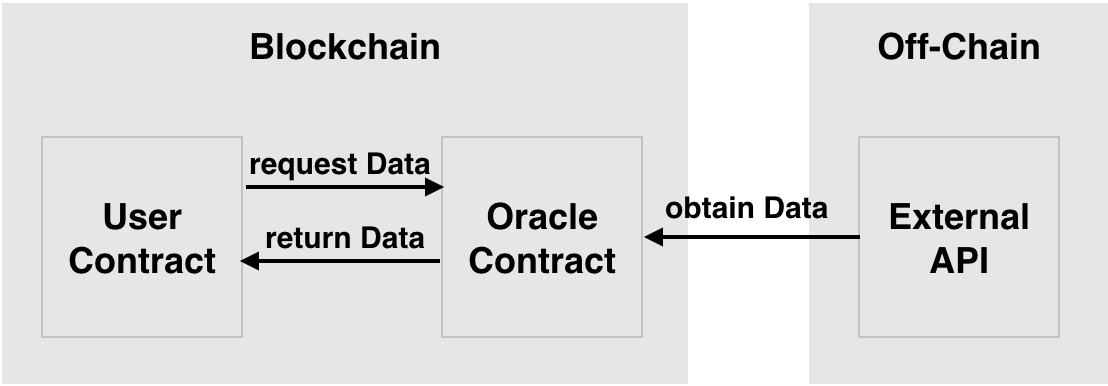
\includegraphics[width=9cm]{idealOracle.png}
		\caption{Ideal oracle workflow}
		\label{idealOracle}
	\end{center}
\end{figure} 
As the request and the result are exchanged on the blockchain, the messages are public, which must be avoided in case of sensitive data. To create a confidential communication, the request from the user contract can be encrypted with the public key of the oracle, ensuring that only the oracle contract can access the information. \cite{Ellis2017} \par
In practice, neither perfectly trustworthy data sources nor reliable third parties can be assumed. Thus, an oracle implementation which can handle unreliable data sources and malicious third parties has to be found. Three different approaches are presented in the following. \cite{Mik2017} 
\subsection{Implementation}
\subsubsection{Decentralized Oracles}
The issue of faulty data sources can be solved by using distributed sources instead of addressing one single API. The oracle will thus receive a multitude of answers and has to aggregate them. This could be done in different ways depending on the type of data. One possibility is majority voting, where the most reported answer is returned. Another could be ignoring the outliners in the data and return the mean of the remaining information. \cite{Mik2017} \cite{Ellis2017} \par 
Besides the data quality, relying on a single party would contradict the idea of the decentralized blockchain and it cannot be assumed that a single oracle is unconditionally trustworthy. Therefore, distributed oracles in form of a decentralized oracle network are introduced. Each oracle addresses a set of data sources and aggregates the information to one result. The oracle network will then find a consensus which ensures that the correct information is reported to the user contract even if some of the oracles in the network are faulty. \cite{Ellis2017} \par 
ChainLink proposes a solution for a decentralized oracle network, which consists of an on-chain and an off-chain part. ChainLink's on-chain interface is used for communicating directly with user contracts on the blockchain and is composed of three main contracts:
\begin{itemize}
	\item Reputation contract: To reward good performing oracles in the network, the reputation contract observes and reports several metrics like the number of completed requests or the average time to respond. The user can specify a list of oracles, which should execute the task, according to their reputation.
	\item Order-matching contract: The list of oracles to execute the query is forwarded to the order-matching contract, which notifies the ChainLink nodes and waits for their response whether they accept the task or not. After the automated oracle matching is completed, the order-matching contract sends a message to the final oracle selection and they start executing the task.
	\item Aggregating contract: The responses of the ChainLink nodes are collected by the aggregating contract, which calculates the result of the query by creating a consensus between the different answers. It also reports the reputation metrics of the participating oracles back to the reputation contract. \cite{Ellis2017}   
\end{itemize}
The on-chain component is for simplicity in the following abstracted to a single "on-chain contract".
The ChainLink off-chain part consists of the oracle network, which communicates with external APIs. Each of the nodes is composed of two modules. The first module is the core, which interfaces the on-chain part of ChainLink. 
\begin{figure}[h]
	\begin{center}
		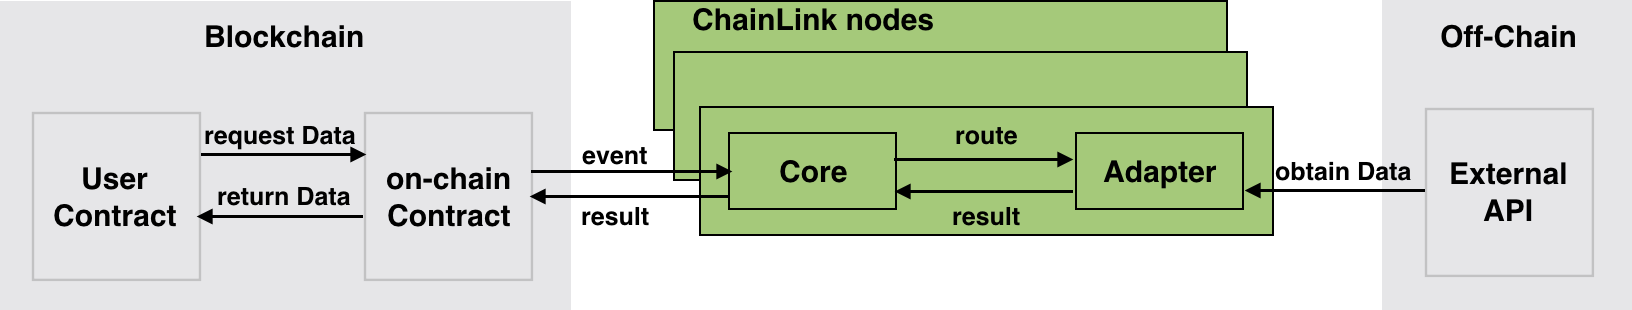
\includegraphics[width=9cm]{ChainLink.png}
		\caption{ChainLink architecture}
		\label{chainlink}
	\end{center}
\end{figure}  
As indicated in \ref{chainlink}, the core receives the event, which was logged by the on-chain contract, to which the request was sent. The core is responsible for scheduling and balancing the events, it will thus route the task to the next module in the node, the adapter. Adapters simplify the interaction with the external API by converting complex multi-step APIs to manageable individual subtasks. After receiving the task, the adapter will obtain the data from the API and send the response back to the core, which reports the data to the on-chain contract. The on-chain contract takes care of delivering the information to the user contract. \cite{Ellis2017} \par 
The above presented solution makes use of in-contract aggregation because all ChainLink nodes report their results individually and the on-chain contract performs the aggregation. An important challenge for this mechanism is called freeloading, which means that an oracle could wait for the responses of other oracles and copy the answer without having to perform the query. To prevent this, a commit / reveal scheme is introduced, where the oracles send encrypted responses to the on-chain contract and after all answers have been delivered, the oracles reveal the data in a second round. \cite{Ellis2017} \par 
It becomes obvious that the costs for transmitting the oracle messages and processing them is a decisive disadvantage of the in-contract aggregation. Off-chain aggregation offers an alternative without having the on-chain contract to participate in the consensus mechanism. For this approach, the oracles have a shared key pair. Sharing in this case means that each node has its own public and private key, which can generate a partial signature. If the same data was partially signed, those can be combined to a single collective signature. The information that succesfully created a valid signature can then be passed on to the on-chain contract, which only has to forward it to the user contract. \cite{Ellis2017} \par
In summary, decentralized oracles like ChainLink provide a high security level. It is not necessary to rely on a single service provider because of the distributed architecture, which ensures the data integrity that is needed to deal with smart contracts. In contrast, the computation in a distributed network is costly because the data has to be aggregated in separate mechanisms and the nodes have to agree on a data format that all nodes can accept. Additionally, even if querys are encrypted for confidentiality, the query has to be decrypted by the oracle service who will then see the query. \cite{Ellis2017} \cite{Oraclize2017}
\subsubsection{Untampered Data Sources}
Web applications can authenticate data with the help of the HTTPS protocol. Blockchain applications like smart contracts do not have the possibility to interact with HTTPS, so there is the need of a service providing authenticated and untempered data. Oracles as untampered data sources provide systems to authenticate data and to proof that the provided data is untempered. \cite{Oraclize2017} \par 
Oraclize is one of the most common oracles \cite{Bartoletti2017}. The main difference to other oracles is that Oraclize returns the requested data together with a document called authenticity proof. With this additional document Oraclize aims to achieve genuine and untampered data purchase. The authenticity proof can be provided by different technologies, for example auditable virtual machines or Trusted Execution Environments. TLSNotary Proof and Android Proof are examples for software-based authenticity proof types and Ledger Proof is based on secure hardware. The authenticity proof may be a large file and providing it directly with the requested data might get expensive. Therefore Oraclize only provides a pointer to the stored authenticity proof in IPFS, a decentralized and distributed storage system. \cite{Oraclize2017} \par
Oraclize is not specialized on a certain smart contract platform but it can be integrated into different blockchain protocols. There are possible applications in various public platforms like Ethereum, Bitcoin, etc. \cite{Oraclize2017}
Oraclize returns data if certain predefined conditions are true. A request to Oraclize needs to contain:
\begin{itemize}
	\item A data source type: The type of data source where Oraclize gains the information from. It can be a website, a web API, a secure application on trusted hardware or a locked-down virtual machine running in a cloud. At the moment Oraclize supports URL (access to  webpage or HTTP API endpoint), WolframAlpha, IPFS (access to content stored on an IPFS file), random (access to untampered random bytes from a secure application running on a Ledger Nano S), computation (access to the result of arbitrary computation).
	\item A query: All parameters which have to be considered when a data request is processes are put together into an array. Each data source type expects different parameters. One parameter of the query when the data source type is URL for example is the URL where the data source resides. If a (interim) result of a query needs to be parsed Oraclize supports XML, JSON, XHTML and a binary parser helpers.
	\item Optionally an authenticity proof type: Oraclize is an untrusted middleman. But on demand users may request an authenticity proof whose (?) type is defined with this parameter. \cite{Oraclize2017}
\end{itemize}
In order to also provide data privacy users of Oraclize may encrypt their queries/parts of it with the Oraclize public key. The service of Oraclize costs a fee depending on the data source type and the authenticity proof type. \cite{Oraclize2017} \par
Even if encryption is possible, the data will be decrypted by the oracle service and therefore visible for the oracle. Additionally, Oraclize as a centralized oracle has the general issue that there is a centralized point of control which leads to problems with tamper resistance. The advantages of Oraclize are that the users and smart contracts do not need to trust Oraclize and that data sources do not need to change anything. With Oraclize the smart contract can gather information from the data sources via APIs or websites directly. \cite{Ellis2017} \cite{Oraclize2017} \par    
\subsubsection{Trusted Hardware}
Another solution for gathering data for smart contracts is trusted hardware. The oracle based on trusted hardware connects a blockchain front end with a trusted hardware back end. There is a connection between a smart contract and a off-chain trusted computer environment. A trusted hardware component is one possible answer to the general issue of smart contracts: The lack of a trustworthy data feed. \cite{Zhang2016} \par 
Trusted hardware is certified hardware to perform in manner of particular requirements. Hardware as cryptographic modules fulfill security requirements to be secure from external attacks. \cite{Sion2009} \par 
An example for this approach is Town Crier. Town Crier connects smart contracts with existing websites which already are commonly trusted for non-blockchain applications. In more detail Twon Crier creates a connection between HTTPS-enabled websites and the Ethereum blockchain and provides an authenticated data feed respectively oracle. It gathers data from the websites and passes it on to the inquiring(??) smart contract in form of so called datagrams. Town Crier is especially developed for the platform Ethereum. Customers have to pay gas fees in form of Ether beforehand to get the requested datagram. \cite{Zhang2016} \par 
Town Crier uses Intel’s SGX - Software Guard Extension as a trusted hardware back end and a smart contract front end. With SGX it is possible to execute processes in an isolated enclave which protects the process from manipulation by hardware attacks and software on the same host, even the operating system. SGX can create a report to verify the software run in the enclave. This report contain the \textit{measurement} (hash of the enclave's initial state), a public key and a digital signature as a hardware-protected key to show that the measured software really run in the SGX-protected enclave. As indicated in \ref{towncrier} the Enclave is one of Town Crier's three main components: The Town Crier Contract C$_{TC}$ (on the blockchain), the Enclave and the Relay (on the Town Crier server). 
\begin{figure}[h]
	\begin{center}
		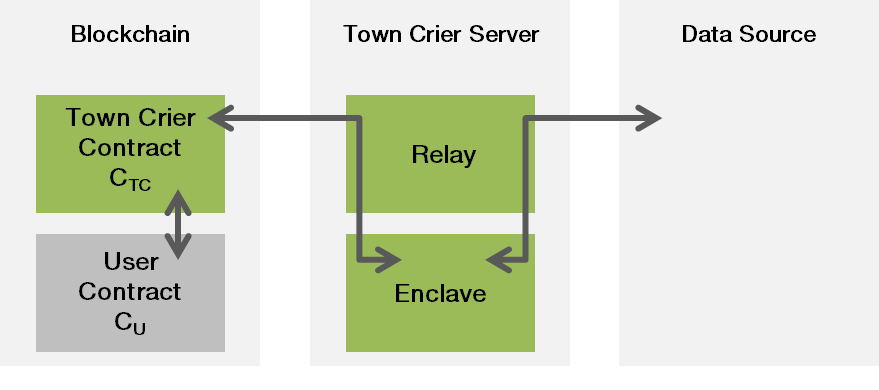
\includegraphics[width=9cm]{TownCrier.png}
		\caption{Town Crier architecture}
		\label{towncrier}
	\end{center}
\end{figure}
The C$_{TC}$ represents a simple API to a requesting smart contract which wants to use Town Crier's services of getting data from a website (called C$_{U}$ in Town Crier's term). C$_{TC}$ is the smart contract front end of Town Crier. It gets the requests from the requester/relying contract C$_{U}$, returns the datagrams from Town Crier and manages Town Crier's monetary resources. The request from C$_{U}$ to C$_{TC}$ is a message containing parameters like for example the url of the target data source, details of the required data, the delivery time, etc. and "callback", where the datagram has to be returned. As already mentioned before the Enclave is the Town Crier code performed in the isolated SGX enclave, thus an SGX enclave process. C$_{TC}$ forwards the request with a new added id and then the task of the Enclave is to gain the requested data from outside the smart contract, mostly from HTTPS-enabled websites. The Enclave generates a pair of private and public key. Before returning the collected data C$_{TC}$ checks if the parameters of the request and response match. Then it returns a digitally signed blockchain message with the collected data as a datagram to C$_{U}$ via C$_{TC}$. The digital signature for message authentication consists of the pair of private and public key. Because of the missing direct network access of the Enclave there is the third main component of Town Crier, the Relay. The Relay connects the Enclave with the network, specially to C$_{TC}$, which neither has a network connection, to the clients with service requests and to the data sources (HTTP-enabled websites). \cite{Zhang2016} \par 
Concerning the security of Town Crier there are some assumptions made. C$_{TC}$ and the source code are visible for all clients, thus they are assumed to be honest and the code is trusted by all participants. Furthermore there is the assumption that the clients trust the websites where they request data from beforehand and that these websites are stable during the certain needed time interval. So the requester C$_{U}$ only needs to trust the security of SGX, the Town Crier code and correctness of data from the specified source in the specified time interval. \cite{Zhang2016} \par 
In addition to normal requests which are visible on the blockchain Town Crier also supports private and custom requests. Private requests make confidentiality possible by encrypting the parameters under a public key. Custom requests also permits Town Crier to gain access-controlled data from for example online accounts. \cite{Zhang2016} \par 
The advantage in contrast to other oracle solutions is encryption in combination with trusted hardware. In trusted hardware oracles queries can be decrypted in the enclave and after the encryption the query is processed within the enclave without any other process having access to it. One examle for this advantage of trusted hardware is Town Crier supporting trading on the Steam gaming platform and thereby creating a secure marketplace. Town Crier uses passwords in a secure way and checks if the ownership of a game changed from seller to buyer. In addition, trusted hardware oracles running in an enclave like Town Crier mostly request data via HTTPS. This also ensures that the provided data is untampered. \cite{Ellis2017} An disadvantage of Town Crier on the other hand is that it connects data sources with the Ethereum blockchain \cite{Zhang2016}. Thus, Town Crier is limited to one smart contract platform.
% An example of a floating figure using the graphicx package.
% Note that \label must occur AFTER (or within) \caption.
% For figures, \caption should occur after the \includegraphics.
% Note that IEEEtran v1.7 and later has special internal code that
% is designed to preserve the operation of \label within \caption
% even when the captionsoff option is in effect. However, because
% of issues like this, it may be the safest practice to put all your
% \label just after \caption rather than within \caption{}.
%
% Reminder: the "draftcls" or "draftclsnofoot", not "draft", class
% option should be used if it is desired that the figures are to be
% displayed while in draft mode.
%
%\begin{figure}[!t]
%\centering
%\includegraphics[width=2.5in]{myfigure}
% where an .eps filename suffix will be assumed under latex, 
% and a .pdf suffix will be assumed for pdflatex; or what has been declared
% via \DeclareGraphicsExtensions.
%\caption{Simulation results for the network.}
%\label{fig_sim}
%\end{figure}

% Note that the IEEE typically puts floats only at the top, even when this
% results in a large percentage of a column being occupied by floats.


% An example of a double column floating figure using two subfigures.
% (The subfig.sty package must be loaded for this to work.)
% The subfigure \label commands are set within each subfloat command,
% and the \label for the overall figure must come after \caption.
% \hfil is used as a separator to get equal spacing.
% Watch out that the combined width of all the subfigures on a 
% line do not exceed the text width or a line break will occur.
%
%\begin{figure*}[!t]
%\centering
%\subfloat[Case I]{\includegraphics[width=2.5in]{box}%
%\label{fig_first_case}}
%\hfil
%\subfloat[Case II]{\includegraphics[width=2.5in]{box}%
%\label{fig_second_case}}
%\caption{Simulation results for the network.}
%\label{fig_sim}
%\end{figure*}
%
% Note that often IEEE papers with subfigures do not employ subfigure
% captions (using the optional argument to \subfloat[]), but instead will
% reference/describe all of them (a), (b), etc., within the main caption.
% Be aware that for subfig.sty to generate the (a), (b), etc., subfigure
% labels, the optional argument to \subfloat must be present. If a
% subcaption is not desired, just leave its contents blank,
% e.g., \subfloat[].


% An example of a floating table. Note that, for IEEE style tables, the
% \caption command should come BEFORE the table and, given that table
% captions serve much like titles, are usually capitalized except for words
% such as a, an, and, as, at, but, by, for, in, nor, of, on, or, the, to
% and up, which are usually not capitalized unless they are the first or
% last word of the caption. Table text will default to \footnotesize as
% the IEEE normally uses this smaller font for tables.
% The \label must come after \caption as always.
%
%\begin{table}[!t]
%% increase table row spacing, adjust to taste
%\renewcommand{\arraystretch}{1.3}
% if using array.sty, it might be a good idea to tweak the value of
% \extrarowheight as needed to properly center the text within the cells
%\caption{An Example of a Table}
%\label{table_example}
%\centering
%% Some packages, such as MDW tools, offer better commands for making tables
%% than the plain LaTeX2e tabular which is used here.
%\begin{tabular}{|c||c|}
%\hline
%One & Two\\
%\hline
%Three & Four\\
%\hline
%\end{tabular}
%\end{table}


% Note that the IEEE does not put floats in the very first column
% - or typically anywhere on the first page for that matter. Also,
% in-text middle ("here") positioning is typically not used, but it
% is allowed and encouraged for Computer Society conferences (but
% not Computer Society journals). Most IEEE journals/conferences use
% top floats exclusively. 
% Note that, LaTeX2e, unlike IEEE journals/conferences, places
% footnotes above bottom floats. This can be corrected via the
% \fnbelowfloat command of the stfloats package.




\section{Conclusion}
In summary, this paper has shown that a smart contract relies on two critical factors, the expression of the contract in code and providing the necessary data. After explaining the basics of smart contracts and the blockchain technology, the most commonly used tools, namely platforms and programming languages, were presented to give an overview of the structure and the technical requirements of smart contracts in the blockchain environment. The analysis of the smart contract implementation made clear that the blockchain remains isolated from the off-chain world, which justifies the necessity of authenticated data feed providers, so called oracles. Three different approaches for oracle implementations, decentralized oracles, untampered data sources and trusted hardware, were explained and evaluated. In comparison, for each current solution there is still improvement possible and needed. Even though a perfect oracle would combine the advantages of all three approaches, this would result in a very complex and costly architecture. From application to application, the imposed requirements on the trade-off between security and costs are different. Therefore, the oracle market should continue providing diverse approaches which fulfill this trade-off in a distict manner.  



% trigger a \newpage just before the given reference
% number - used to balance the columns on the last page
% adjust value as needed - may need to be readjusted if
% the document is modified later
%\IEEEtriggeratref{8}
% The "triggered" command can be changed if desired:
%\IEEEtriggercmd{\enlargethispage{-5in}}

% references section

% can use a bibliography generated by BibTeX as a .bbl file
% BibTeX documentation can be easily obtained at:
% http://mirror.ctan.org/biblio/bibtex/contrib/doc/
% The IEEEtran BibTeX style support page is at:
% http://www.michaelshell.org/tex/ieeetran/bibtex/
\bibliographystyle{IEEEtran}
% argument is your BibTeX string definitions and bibliography database(s)
\bibliography{Literatur}
%
% <OR> manually copy in the resultant .bbl file
% set second argument of \begin to the number of references
% (used to reserve space for the reference number labels box)





% that's all folks
\end{document}


